\chapter{Results}

During the experiment, some interesting properties were assessed using the 
survey paper while other parameters were recorded by the Android application. 
This chapter aims to collect, classify and analyze these records to 
achieve 3 objectives. First, to confirm or reverse the hypotheses, then 
possibly to formulate new hypotheses and finally to assess the usability of 
new menu organizations. As explained earlier, usability is measured with 3 
interesting properties: (1)  effectiveness, (2) efficiency and (3) 
satisfaction. This section first describes the participants who took part to 
the experiment and then analyzes these usability-related properties one after 
the other. The hypotheses are finally discussed at the end of the chapter.

\section{Participants}

The study was conducted with 18 French speaking subjects between 17 and 61 
years old. To avoid bias due to language, the application and the survey 
used during the experiment were translated in French. Moreover, the experiment 
has been conducted with the same smartphone for each participant. The 
smartphone was a Sony Xperia M2 with a 4.8 inches screen. Half the 
participants were men while the other half was women. Parity gender was 
therefore achieved.\newline

The subjects come from various backgrounds that we have grouped in 4 
distinct categories: (1) engineers, (2) art school students/workers, (3) other 
academics, and (5) others. \textit{Engineers} and \textit{art school 
students/workers} were enough to get their own representative 
category. \textit{Other academics} consisted of 1 law student, 1 foreign 
language student, 1 psychology student and 1 physical education student. 
Finally, 2 administrative employees, 1 worker, 1 saleswoman and 1 pupil were 
part of the last category called \textit{others}. Figure \ref{fig:participants} 
(a) depicts the distribution of participants according to their educational 
background. It also highlights the distribution of men and women among these 
categories. Notice that men are mainly representing engineering and artistic 
careers in our participant sample. Women are mostly representing other academics 
and other careers. Unfortunately, the parity gender is not well represented by 
a distribution based on the educational background.

\begin{figure}[!ht]
    
  \begin{subfigure}[t]{.49\textwidth}
  \centering
  \resizebox{\linewidth}{!}{
  \begin{tikzpicture}[baseline]
    \begin{axis}[
      %title={Evolution of student participation for each exercise},
      enlarge y limits=false,
      axis lines*=left,
      %xlabel={Educational background},
      ylabel={\# participants},
      %xmin=1, xmax=4,
      ymin=1, ymax=6,
      xtick=data,
      ytick={1,2,3,4,5,6},
      legend pos=east,
      legend columns=0,
      %xmajorgrids=true,
      ymajorgrids=true,
      grid style=dashed,
      enlargelimits=0.15,
      %histogram related :
      ybar,
      symbolic x coords={engineers, art school, other academics, others},
      nodes near coords,
      xticklabel style={
	inner sep=0pt,
	anchor=north east,
	rotate=45
      }
      ]
      
    \addplot[blue!50!black, fill=blue!55] coordinates
    {(engineers, 4) (art school, 3) (other academics, 1) (others, 1)};   
    \addplot[red!70!black, fill=red!35] coordinates
    {(engineers, 1) (art school, 1) (other academics, 3) (others, 4)}; 
    
    \legend{Men, Women}
    
    \end{axis}
  \end{tikzpicture}}
  \caption{Distribution of participants according to their educational 
background.}
  \label{fig:background}
  \end{subfigure}
  \begin{subfigure}[t]{.49\textwidth}
    \resizebox{\linewidth}{!}{
    \centering
    \begin{tikzpicture}[baseline]
    \begin{axis}[
      %title={Evolution of student participation for each exercise},
      enlarge y limits=false,
      axis lines*=left,
      xlabel={Age group},
      ylabel={\# participants},
      %xmin=1, xmax=4,
      ymin=1, ymax=6,
      xtick=data,
      ytick={1,2,3,4,5,6},
      legend pos=east,
      legend columns=0,
      %xmajorgrids=true,
      ymajorgrids=true,
      grid style=dashed,
      enlargelimits=0.15,
      %histogram related :
      ybar,
      symbolic x coords={<25, 25-40, >40 years old},
      nodes near coords,
      ]
      
    \addplot[blue!50!black, fill=blue!55] coordinates
    {(<25, 5) (25-40, 2) (>40 years old, 2)};   
    \addplot[red!70!black, fill=red!35] coordinates
    {(<25, 4) (25-40, 2) (>40 years old, 3)};
    
    \legend{Men, Women}
    
    \end{axis}
  \end{tikzpicture}}
  \caption{Distribution of participants according to their age group.}
  \label{fig:age_range}
  \end{subfigure}
  \caption{}
    \label{fig:participants}
\end{figure}

Figure \ref{fig:participants} (b) depicts the distribution 
of participants according to their age group. It also highlights gender 
distribution. Most participants were between 18 and 25 but each age group was 
at 
least represented once during the experiment. We were able to form and use the 
3 
following groups of participants during the analysis: (1) <25, (2) 25-40 and 
(3) >40 years old. Parity gender is very well represented among these 
categories. Therefore it can be appropriate to distinguish gender and age groups 
during the analysis.\newline

Participants were also asked to rate their skills with smartphones and 
touch screen technologies. The objective was to differentiate 2 groups of 
subjects: (1) novice and (2) master users. Unfortunately, smartphone users 
and touch screens are becoming more common nowadays and we haven't found 
enough novice users for the experiment. Even subjects without smartphones 
considered themselves rather efficient with touch screens and smartphones. 
Therefore, we will not be able to prove the hypothesis based on novice 
users and their preference for adaptive menus. Figure 
\ref{fig:participants_skills} illustrates the distribution of participants' 
responses about their skills with smartphones and 
touch screens. Notice that a rating ranging from 1 (bad) to 7 (excellent) was 
at their disposal to assess their abilities.

\begin{figure}[!ht]
      \centering
  \begin{tikzpicture}
    \begin{axis}[
      %title={Evolution of student participation for each exercise},
      width=11cm,
      enlarge y limits=false,
      axis lines*=left,
      xlabel={Rating},
      ylabel={\# participants},
      xmin=1, xmax=7,
      ymin=1, ymax=10,
      xtick=data,
      ytick={0,1,2,3,4,5,6,7,8,9,10},
      legend pos=east,
      legend columns=0,
      %xmajorgrids=true,
      ymajorgrids=true,
      grid style=dashed,
      enlargelimits=0.15,
      %histogram related :
      ybar,
      symbolic x coords={1,2,3,4,5,6,7},
      nodes near coords,
      ]
      
    \addplot[green!40!black, fill=green!65] coordinates
    { (1,0) (2,1) (3,2) (4,2) (5,3) (6,1) (7,9)};   
    \addplot[orange!70!black, fill=orange!30] coordinates
    { (1,0) (2,1) (3,1) (4,0) (5,4) (6,3) (7,9)};
    
    \legend{w/ Smartphone, w/ Touch screen}
    
    \end{axis}
  \end{tikzpicture}
  \caption{Distribution of participants according to their own estimations of 
their skills with smartphones and touch screens.}
  \label{fig:age_range}
    \label{fig:participants_skills}
\end{figure}

\section{Effectiveness}
Effectiveness is the first property to evaluate in order to assess the 
usability of a menu organization. According to the Oxford English Dictionary, 
effectiveness can be defined as \enquote{the degree to which something is 
successful in producing a desired result; success} \cite{effectiveness}. In 
1998, effectiveness was defined more precisely by HCI researchers in 
the ISO9241-11 standard which describes it as \enquote{the accuracy and 
completeness of users' 
tasks while using a system} \cite{iso}. Indeed, when using the 
menu of a computer system, a user wishes to fulfill a precise action - e.g. 
saving a document - and must press the related menu item - e.g. the button 
\enquote{save} - in order 
to execute this action. In other words, the effectiveness of a menu 
organization can be assessed by observing its average error rate. A low error 
rate means that users have managed to produce the desired results by pressing 
the correct buttons during the experiment. The control condition menu 
displayed 
by \textit{MenuActivity} can be used to benchmark the effectiveness between 
menu organizations. A lower error rate than \textit{MenuActivity} means that 
the users have managed to produce the desired results more frequently with new 
menu 
organizations.\newline

Figure \ref{fig:errors} (a) depicts the average error rate for each 
menu organization. The control condition menu (1) and the split menu (3) seem 
to be the worst menu organizations in terms of effectiveness. The new menu 
organizations showed better results as users achieved lower error rates when 
using them. Even more interesting, the users did not commit any mistake when 
using the responsive menu (5). However, notice that the worst 
average error rate does not even exceed $3.33\%$. In conclusion, all 
the displayed menu organizations can be considered as greatly effective.

\begin{figure}[!ht]
    
  \begin{subfigure}[t]{.49\textwidth}
  \centering
  \resizebox{\linewidth}{!}{
  \begin{tikzpicture}[baseline]
    \begin{axis}[
      %title={Evolution of student participation for each exercise},
      enlarge y limits=false,
      axis lines*=left,
      xlabel={Menu organization},
      ylabel={Average error rate (\%)},
      xmin=1, xmax=8,
      ymin=1, ymax=10,
      xtick=data,
      %ytick={0,1,2,4},
      legend pos=east,
      legend columns=0,
      %xmajorgrids=true,
      ymajorgrids=true,
      grid style=dashed,
      enlargelimits=0.15,
      %histogram related :
      ybar,
      symbolic x coords={1,2,3,4,5,6,7,8},
      nodes near coords,
      ]
      
    \addplot[orange!70!black, fill=orange!30] coordinates
    {(1,3.3333) (2,0.5556) (3,3.3333) (4,1.6667) (5,0) (6,1.6667) (7,1.1111) 
     (8,0.5556)};
    
    %\legend{Men, Women}
    
    \end{axis}
  \end{tikzpicture}}
  \caption{Average error rate for each menu organization.}
  \label{fig:background}
  \end{subfigure}
  \begin{subfigure}[t]{.49\textwidth}
    \resizebox{\linewidth}{!}{
    \centering
    \begin{tikzpicture}[baseline]
    \begin{axis}[
      %title={Evolution of student participation for each exercise},
      enlarge y limits=false,
      axis lines*=left,
      xlabel={Age group},
      ylabel={Average error rate (\%)},
      %xmin=1, xmax=4,
      ymin=1, ymax=10,
      xtick=data,
      %ytick={1,2,3,4,5,6},
      legend pos=east,
      legend columns=0,
      %xmajorgrids=true,
      ymajorgrids=true,
      grid style=dashed,
      enlargelimits=0.15,
      %histogram related :
      ybar,
      symbolic x coords={<25, 25-40, >40 years old},
      nodes near coords,
      ]
      
    \addplot[blue!50!black, fill=blue!55] coordinates
    {(<25, 2.8) (25-40, 0) (>40 years old, 1.9)};   
    \addplot[red!70!black, fill=red!35] coordinates
    {(<25, 0) (25-40, 1.3) (>40 years old, 2.5)};
    
    \legend{Men, Women}
    
    \end{axis}
  \end{tikzpicture}}
  \caption{Average error rate according to the age group and the gender 
distinction.}
  \label{fig:age_range}
  \end{subfigure}
  \caption{}
    \label{fig:errors}
\end{figure}

Figure \ref{fig:errors} (b) depicts the average error rate according to 
the age group. It also highlights gender distinction and shows that men are 
slightly less effective than women. In general, they commit more mistakes than 
women. However, women tend to commit more and more errors over the years. Older 
participants show the worst average error rate while the intermediary age group 
shows the best average error rate.

\begin{figure}[!ht]
    \centering
\begin{tikzpicture}
    \begin{axis}[
      %title={Evolution of student participation for each exercise},
      enlarge y limits=false,
      enlarge x limits=-1,
      height=6cm,
      width=14.5cm,
      axis lines*=left,
      xlabel={Participant id},
      ylabel={\# errors},
      xmin=1, xmax=18,
      ymin=0, ymax=6,
      xtick=data,
      ytick={0,1,2,3,4,5,6},
      legend pos=east,
      legend columns=0,
      %xmajorgrids=true,
      ymajorgrids=true,
      grid style=dashed,
      enlargelimits=0.15,
      %histogram related :
      ybar,
      symbolic x coords={1,2,3,4,5,6,7,8,9,10,11,12,13,14,15,16,17,18},
      nodes near coords,
      ]
      
    \addplot[orange!70!black, fill=orange!40] coordinates
    {(1,1) (2,0) (3,2) (4,0) (5,0) (6,2) (7,1) (8,5) (9,1) (10,4) (11,1) (12,0)
     (13,0) (14,2) (15,0) (16,2) (17,1) (18,0)};
    
    %\legend{Men, Women}
    
    \end{axis}
  \end{tikzpicture}
  \caption{Number of errors performed by each participant after 80 
selections.}
    \label{fig:errors_participants}
\end{figure}

It is finally interesting to observe more precisely the errors performed during 
the experiment. Figure \ref{fig:errors_participants} 
illustrates the distribution of errors among the subjects of the 
experiment. We can first notice that nearly half the mistakes were 
performed by 2 participants. These subjects made 4 and 5 errors 
which is respectively 4 and 5 times greater than the average number of 
mistakes performed by each participant. A deeper analysis of mistakes 
allowed us to identify 4 types of errors: (1) forgetting, (2) touch screen 
imprecision, (3) inattention and (4) confusion. Some participants complained 
about \textit{forgetting} the required item because it disappeared once the menu 
was displayed. The problem occured 9 times as illustrated by Figure 
\ref{fig:errors_types}. It corresponds to nearly half the mistakes performed 
during the study. The \textit{imprecision} mistake also occured a few times. It 
happened when subjects ended up pressing on a button instead of scrolling down 
the menu, or when they ended up pressing on a button above or below the 
desired item. The \textit{inattention} error occured when 
the hot list of a split menu was updated and users were not attentive enough to 
these changes. Therefore, they ended up pressing on a wrong button. Finally, 
\textit{confusion} happened a few times between the words \enquote{Germany} and 
\enquote{England}, and \enquote{Walnut} and \enquote{Pecan} due to the fact that 
these words are pretty close to each other in french (Allemagne/Angleterre and 
Noix/Noix de Pecan).

\begin{figure}[!ht]
    \centering
\begin{tikzpicture}
    \begin{axis}[
      %title={Evolution of student participation for each exercise},
      enlarge y limits=false,
      enlarge x limits=-1,
      height=6cm,
      width=14.5cm,
      axis lines*=left,
      xlabel={Type of mistake},
      ylabel={\# errors},
      %xmin=1, xmax=4,
      ymin=0, ymax=10,
      xtick=data,
      ytick={0,2,4,6,8,10},
      legend pos=east,
      legend columns=0,
      %xmajorgrids=true,
      ymajorgrids=true,
      grid style=dashed,
      enlargelimits=0.15,
      %histogram related :
      ybar,
      symbolic x coords={forgetting, imprecision, inattention, confusion},
      nodes near coords,
      ]
      
    \addplot[orange!70!black, fill=orange!30] coordinates
    {(forgetting,9) (imprecision,6) (inattention,4) (confusion,3)};
    
    %\legend{Men, Women}
    
    \end{axis}
  \end{tikzpicture}
  \caption{Distribution of errors among the 4 identified types of mistakes.}
    \label{fig:errors_types}
\end{figure}

\section{Efficiency}
Effiency is the second interesting property to observe when assessing menu 
usability. According to the Oxford English Dictionary, efficiency is defined as 
\enquote{the ratio of the useful work performed by a machine or in a process to 
the total energy expended or heat taken in} \cite{efficiency}. In 1998, HCI 
researchers defined the term more rigourously with the ISO9241-11 standard. 
They described it as \enquote{the resources expended by the user in relation to 
the 
accuracy and completeness of goals achieved} \cite{iso}. In other 
words, a computer system is said to be efficient if users manage to reach 
their goals while expending as little resources as possible. Therefore, we 
should 
focus on observing lower selection time for new menu organizations compared to 
the 
control condition menu. It is also relevant to adopt a \textit{productivity} 
approach such that we can observe the ratio of successful selection rate 
(useful output) to average required selection time (input). Figure 
\ref{fig:selectime} (a) depicts the average selection time for 
each menu organization. It shows that all menu organizations reduce the 
selection time in comparison to the control condition menu (1), except for the 
minimised menu (2) which slightly increases this value. The responsive 
menu (5) is once again the most performant one. Figure 
\ref{fig:selectime} (b) illustrates the productivity ratio for each menu 
organization. All menu organizations can be considered as more efficient than 
the traditional menu. The productivity approach also confirms that the 
responsive menu is the most performant one. Indeed, it provides the best 
results 
in terms of effectiveness (lower error rate) and efficiency (lower selection 
time).

\begin{figure}[!ht]
    
  \begin{subfigure}[t]{.49\textwidth}
  \centering
  \resizebox{\linewidth}{!}{
  \begin{tikzpicture}[baseline]
    \begin{axis}[
      %title={Evolution of student participation for each exercise},
      enlarge y limits=false,
      axis lines*=left,
      xlabel={Menu organization},
      ylabel={Average selection time (s)},
      xmin=1, xmax=8,
      ymin=2, ymax=3,
      xtick=data,
      ytick={2,2.2,2.4,2.6,2.8,3},
      legend pos=east,
      legend columns=0,
      %xmajorgrids=true,
      ymajorgrids=true,
      grid style=dashed,
      enlargelimits=0.15,
      %histogram related :
      ybar,
      symbolic x coords={1,2,3,4,5,6,7,8},
      nodes near coords,
      ]
      
    \addplot[orange!70!black, fill=orange!30] coordinates
    {(1,2.497) (2,2.517) (3,2.464) (4,2.260) (5,2.067) (6,2.314) (7,2.351) 
     (8,2.322)};
    
    %\legend{Men, Women}
    
    \end{axis}
  \end{tikzpicture}}
  \caption{Average selection time for each menu organization.}
  \label{fig:background}
  \end{subfigure}
  \begin{subfigure}[t]{.49\textwidth}
    \resizebox{\linewidth}{!}{
    \centering
    \begin{tikzpicture}[baseline]
    \begin{axis}[
      %title={Evolution of student participation for each exercise},
      enlarge y limits=false,
      axis lines*=left,
      xlabel={Menu organization},
      ylabel={Prod. (success rate/selection time)},
      xmin=1, xmax=8,
      ymin=30, ymax=55,
      xtick=data,
      ytick={30,35,40,45,50,55},
      legend pos=east,
      legend columns=0,
      %xmajorgrids=true,
      ymajorgrids=true,
      grid style=dashed,
      enlargelimits=0.15,
      %histogram related :
      ybar,
      symbolic x coords={1,2,3,4,5,6,7,8},
      nodes near coords,
      every node near coord/.append style={
	  /pgf/number format/fixed zerofill,
	  /pgf/number format/precision=1
      }
      ]
      
    \addplot[green!40!black, fill=green!65] coordinates
    {(1,38.707) (2,39.514) (3,39.37) (4,43.515) (5,48.371) (6,42.494)
     (7,42.063) (8,42.834)};
    
    %\legend{Men, Women}
    
    \end{axis}
  \end{tikzpicture}}
  \caption{Productivity ratio for each menu organization.}
  \label{fig:selectime}
  \end{subfigure}
  \caption{}
    \label{fig:selectime}
\end{figure}

Figure \ref{fig:selectime_agegender} depicts the productivity according 
to the age group and highlights gender distinction. It is first 
interesting to notice that younger participants are more productive 
than older ones. In average, men are also more productive than women. We 
observed in the previous section that women are more effective than men 
because they are performing less mistakes. However, men perform selection 
faster than women and therefore their productivity ratio is slightly 
better.

\begin{figure}[!ht]
    \centering
\begin{tikzpicture}
    \begin{axis}[
      %title={Evolution of student participation for each exercise},
      enlarge y limits=false,
      enlarge x limits=-1,
      height=6cm,
      width=14.5cm,
      axis lines*=left,
      xlabel={Age group},
      ylabel={Prod. (success rate/selection time)},
      %xmin=1, xmax=4,
      ymin=30, ymax=55,
      xtick=data,
      ytick={30,35,40,45,50,55},
      legend pos=east,
      legend columns=0,
      %xmajorgrids=true,
      ymajorgrids=true,
      grid style=dashed,
      enlargelimits=0.15,
      %histogram related :
      ybar,
      symbolic x coords={<25, 25-40, >40 years old},
      nodes near coords,
      every node near coord/.append style={
	  /pgf/number format/fixed zerofill,
	  /pgf/number format/precision=1
      }
      ]
      
    \addplot[blue!50!black, fill=blue!55] coordinates
    {(<25,49.155) (25-40, 46.329) (>40 years old, 33.903)};
    \addplot[red!70!black, fill=red!35] coordinates
    {(<25,53.150) (25-40, 45.827) (>40 years old, 31.399)};
    
    \legend{Men, Women}
    
    \end{axis}
  \end{tikzpicture}
  \caption{Productivity ratio according to the age group and the gender 
distinction.}
    \label{fig:selectime_agegender}
\end{figure}

\section{Satisfaction}
Usability is finally and mostly influenced by user satisfaction. Subjects may 
feel productive but uncomfortable with a given menu organization and its 
underlying operation. The survey paper was mainly focused on gathering users' 
thoughts. The idea was to evaluate how each user was personally 
\textit{feeling} 
and \textit{perceiving} each menu. There are 6 interesting sentences from 
the survey paper useful to assess user satisfaction:
\begin{enumerate}
  \item I felt productive using this menu.
  \item I found this menu easy to use.
  \item I think this menu requires some improvement.
  \item I found this menu well integrated into the smartphone.
  \item I noticed some problems with this menu.
  \item I was frustrated by the menu design.
\end{enumerate}
Subjects had to rate each sentence with a value ranging from 1 (disagree) 
to 7 (agree). Figure \ref{fig:satisfaction_ratio} illustrates the average 
satisfaction ratio for each menu organization. First, a satisfaction ratio was 
computed for each participant and for each menu organization. This ratio 
comprised the values expressed by the participant for each sentence and was 
returned on a scale of 7. The 3rd, 5th and 6th sentence values were inversed 
because agreeing with the fact that a menu requires some improvement, contains 
problems or is frustrating to use is negative for user satisfaction. It is also 
interesting to notice that values from 3 participants were considered as 
invalid. Indeed, they responded with the value 7 for each sentence of the 
survey. Finally, the average satisfaction ratio was computed for each menu 
organization in order to gather all ratios into a single one. This final ratio 
proves that subjects were in general mostly satisfied by the menus designed for 
the experiment. The control condition menu was perceived as the most satisfying 
while the responsive split menu (6) and the minimised responsive split menu (8) 
were perceived as the less satisfying menu organizations. The responsive menu 
(5) which showed great effiency and great effectiveness in the previous sections 
also received a very good satisfaction ratio. Figure 
\ref{fig:satisfaction_gender} depicts the average satisfaction ratio for each 
menu organization and it highlights the gender distinction. It shows that men 
were more satisfied than women about new menu organizations. The 
traditional menu (1) received a better satisfaction from women instead.

\begin{figure}[!ht]
    \centering
\begin{tikzpicture}
    \begin{axis}[
      %title={Evolution of student participation for each exercise},
      enlarge y limits=false,
      enlarge x limits=-1,
      height=6cm,
      width=14.5cm,
      axis lines*=left,
      xlabel={Menu organization},
      ylabel={Average satisfaction ratio},
      %xmin=1, xmax=4,
      ymin=1, ymax=7,
      xtick=data,
      ytick={1,2,3,4,5,6,7},
      legend pos=east,
      legend columns=0,
      %xmajorgrids=true,
      ymajorgrids=true,
      grid style=dashed,
      enlargelimits=0.15,
      %histogram related :
      ybar,
      symbolic x coords={1,2,3,4,5,6,7,8},
      nodes near coords,
      ]
      
    \addplot[orange!70!black, fill=orange!30] coordinates
    {(1,6.04) (2,5.45) (3,5.57) (4,5.42) (5,5.82) (6,5.13) (7,5.65) (8,5.16)};
    
    %\legend{Men, Women}
    
    \end{axis}
  \end{tikzpicture}
  \caption{Average satisfaction ratio for each menu organization.}
    \label{fig:satisfaction_ratio}
\end{figure}

\begin{figure}[!ht]
    \centering
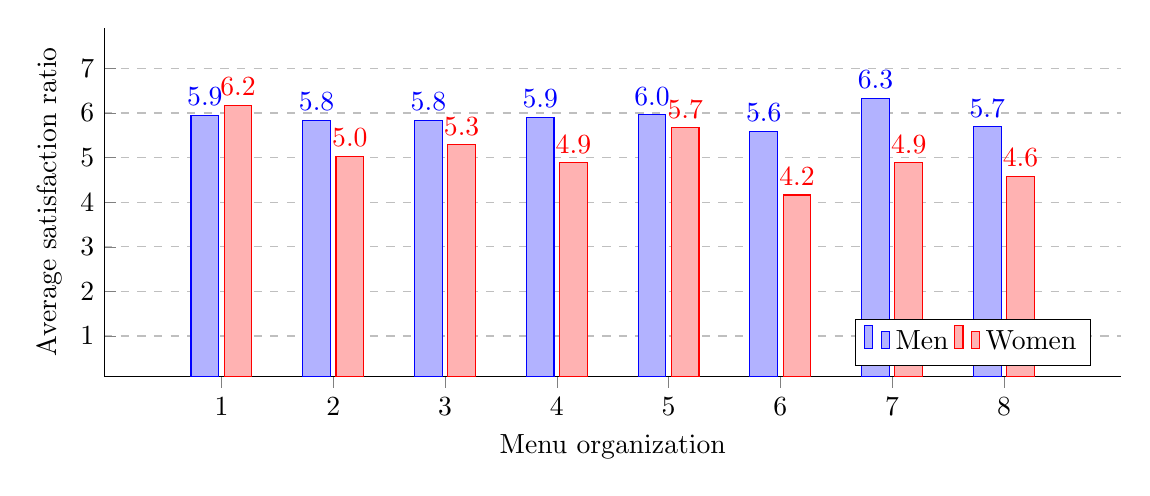
\begin{tikzpicture}
    \begin{axis}[
      %title={Evolution of student participation for each exercise},
      enlarge y limits=false,
      enlarge x limits=-1,
      height=6cm,
      width=14.5cm,
      axis lines*=left,
      xlabel={Menu organization},
      ylabel={Average satisfaction ratio},
      %xmin=1, xmax=4,
      ymin=1, ymax=7,
      xtick=data,
      ytick={1,2,3,4,5,6,7},
      legend pos=south east,
      legend columns=0,
      %xmajorgrids=true,
      ymajorgrids=true,
      grid style=dashed,
      enlargelimits=0.15,
      %histogram related :
      ybar,
      symbolic x coords={1,2,3,4,5,6,7,8},
      nodes near coords,
      every node near coord/.append style={
	  /pgf/number format/fixed zerofill,
	  /pgf/number format/precision=1
      }
      ]
      
    \addplot coordinates
    {(1,5.9375) (2,5.8333) (3,5.8333) (4,5.8958) (5,5.9583) (6,5.5833) 
     (7,6.3333) (8,5.6875)};
    \addplot coordinates
    {(1,6.1666) (2,5.0238) (3,5.2857) (4,4.8809) (5,5.6666) (6,4.16190) 
     (7,4.8809) (8,4.5714)};
    
    \legend{Men, Women}
    
    \end{axis}
  \end{tikzpicture}
  \caption{Average satisfaction ratio for each menu organization according to 
the gender distinction.}
    \label{fig:satisfaction_gender}
\end{figure}

At the end of the experiment, participants were asked to \textit{rank} the menu 
organizations in order of preference and such that a menu ranked at the first 
place was considered as the most preferred menu by the subject. Figure 
\ref{fig:rankings} depicts the average ranking received by each menu 
organization. The traditional (1) and responsive menus (5) were mostly 
preferred by the subjects of the experiment. The responsive minimised split 
menu (8) was by far the less preferred menu. It was ranked by 10 participants as 
the worst menu organization.

\begin{figure}[!ht]
    \centering
\begin{tikzpicture}
    \begin{axis}[
      %title={Evolution of student participation for each exercise},
      enlarge y limits=false,
      enlarge x limits=-1,
      height=6cm,
      width=14.5cm,
      axis lines*=left,
      xlabel={Menu organization},
      ylabel={Average ranking},
      %xmin=1, xmax=4,
      ymin=1, ymax=8,
      xtick=data,
      ytick={1,2,3,4,5,6,7,8},
      legend pos=east,
      legend columns=0,
      %xmajorgrids=true,
      ymajorgrids=true,
      grid style=dashed,
      enlargelimits=0.15,
      %histogram related :
      ybar,
      symbolic x coords={1,2,3,4,5,6,7,8},
      nodes near coords,
      ]
      
    \addplot[orange!70!black, fill=orange!30] coordinates
    {(1,2.7) (2,4.1) (3,4.2) (4,5.6) (5,2.9) (6,4.9) (7,4.9) (8,6.7)};
    
    %\legend{Men, Women}
    
    \end{axis}
  \end{tikzpicture}
  \caption{Average ranking received by each menu organization.}
    \label{fig:rankings}
\end{figure}

\section{Confirming, reversing and updating hypotheses}
The objective of the experiment was to confirm or reverse an initial set of 
11 hypotheses. The results analyzed in the previous sections have led us to 
undertake interesting observations. This section finally aims to confirm, 
reverse and update the initial assumptions based on these observations in order 
to conclude our study.

\subsection{Hypotheses and usability}
In the previous sections, we performed an in-depth analysis of 3 
usability-related properties: (1) effectiveness, (2) efficiency and (3) 
satisfaction. Effectiveness was measured by comparing the average error rate 
between the control condition menu and the new menu organizations. Therefore, 
this property will help us to confirm or reverse hypotheses based on the fact 
that some menu organizations may \textit{reduce the error rate}. The efficiency 
analysis was based on identifying \textit{selection time reduction} and 
eventually \textit{productivity enhancement}. Finally, user satisfaction was 
measured for and between each menu organization. It helped us to identify 
\textit{user preference} for some menu organizations.\newline

Selection time and user preference were already mentioned by the 11 initial 
hypotheses. Two types of hypothesis must now be added up to each 
menu organization. These assumptions are about error rate and productivity 
which were not taken into account at the beginning of our study. These 
additional hypotheses are formulated below:

\begin{itemize}
 \item \textbf{H1c:} the split menu reduces the error rate.
 \item \textbf{H1d:} the split menu enhances the productivity.
 \item \textbf{H2c:} the minimised menu reduces the error rate.
 \item \textbf{H2d:} the minimised menu enhances the productivity.
 \item \textbf{H3c:} the responsive menu reduces the error rate.
 \item \textbf{H3d:} the responsive menu enhances the productivity.
\end{itemize}


\subsection{Split menu}
In 1994, \textsc{Sears} and \textsc{Shneiderman} proved that split menu 
helped to reduce the selection time and received a greater user preference for 
desktop computer system. Unfortunately, our experiment based on 
mobile systems did not show promising results. During the experiment, the split 
menu provided the same average error rate than a traditional menu ($3.33\%$). 
It appears that it also slightly increased the average selection time ($2.52s$ 
instead of $2.5s$ for the control condition menu). Khalid 
\textsc{Al-Omar} and Dimitrios \textsc{Rigas} already experienced the 
same results with their small menu.\newline

In conclusion, the split menu does \textit{not} reduce the error rate, nor the 
selection time in the presence of a mobile system. It was also \textit{not} 
preferred over the traditional menu. Therefore, all the hypotheses based on the 
split menu have to be reversed.

\subsection{Minimised menu}
The minimised menu was meant to help users to identify the desired item 
quicker by reducing the number of displayed items. At first glance, the 
experiment showed promising results. Indeed, the minimised menu provided the 
second lowest average error rate with $0.56\%$ only. Unfortunately, this menu 
organization did not allow to reduce the selection time. The productivity of 
users was slightly increased but still remains unsignificant to be recognized. 
Finally, users were satisfied by the minimised menu organization but did not 
prefer it over the traditional menu.\newline

In conclusion, the minimised menu help users to reduce their error rate. 
However, it is not sufficient to reduce their selection time, nor their 
productivity, and it was not recognized as a preference. Therefore, we are 
only able to confirm one hypothesis:

\begin{itemize}
 \item \textbf{H2c:} the minimised menu reduces the error rate.
\end{itemize}

\subsection{Responsive menu}
Yusuke \textsc{Fukazawa} was the first researcher to publish results based on a 
a responsive menu organization. The idea was to adapt the menu organization to 
the small size of mobile screens. The responsive menu provided great results. 
First, the participants managed to achieve a $0\%$ average error rate by using 
this new 
menu organization. They also achieved the lowest average selection time and 
therefore, the highest productivity ratio. The responsive menu received the 
better satisfaction ratio along with the traditional menu and was preferred 
over all menu organizations.\newline

In conclusion, we managed to prove the 4 hypotheses formulated about responsive 
menus:

\begin{itemize}
 \item \textbf{H3a:} the responsive menu reduces the selection time.
 \item \textbf{H3b:} the responsive menu is preferred by users.
 \item \textbf{H3c:} the responsive menu reduces the error rate.
 \item \textbf{H3d:} the responsive menu enhances the productivity.
\end{itemize}

\subsection{Novice and master users}
Yusuke \textsc{Fukazawa} also noticed that novice and master users usually 
express different preferences regarding new menu organizations. Unfortunately, 
the participants of the experiment were mainly master and frequent smartphone 
users. Therefore, we can only prove the assumptions made on the master 
users and we have to dismiss the assumptions about the novices. Eventhough 
these frequent users expressed a great satisfaction to all menu organizations, 
they mainly ranked the traditional and responsive menus as their favorite 
ones.\newline

In conclusion, we can only confirm and update one hypothesis:

\begin{itemize}
 \item \textbf{H4b:} master users show a preference for the traditional and 
the responsive menus.
\end{itemize}

\subsection{Guidance informations and period of adjustment}
The survey paper was also used to gather users' thoughts about the guidance 
informations and the period of adjustment. There were 3 interesting sentences 
to analyze the impact of these notions on menu usability. Each sentence had to 
be rated on a scale ranging from 1 (disagree) to 7 (agree) for each menu 
organization. These sentences are listed below:

\begin{enumerate}
 \item I found this menu presented as expected.
 \item I needed to learn more this menu.
 \item I needed more guidance informations about this menu.
\end{enumerate}

The 1st and last sentences are helpful to assess the quality of the guidance 
informations provided at the beginning of each training session. Figure 
\ref{fig:guidance} depicts the average rating received for these sentences for 
each menu organization. According to these ratings, the subjects of the 
experiment were very satisfied by the quality of the guidance informations. 
They found menus were all organized as expected and guidance informations were 
sufficient for them to understand new menu organizations.\newline

During the experiment, the participants were first able to train themselves 
with each menu organization for 2 consecutive selections only. Then, they were 
asked if this period of adjustment was long enough according to them. The 
second sentence described above is interesting to evaluate this objective. 
Figure \ref{fig:period} depicts the average rating received for this sentence 
for each menu organization. The results are very prositive. Indeed, users have 
agreed to rate the period of adjustment long enough for all menu 
organizations.\newline

In conclusion, the guidance informations and the period of adjustment have been 
widely appreciated by the participants of the experiment. However we haven't 
tested the experiment without these notions. Therefore, we cannot take proper 
conclusions on the fact that they help users to handle a menu organization more 
efficiently. Since users appreciated the quantity and quality of the provided 
guidance informations, we can only prove the following hypothesis:

\begin{itemize}
 \item \textbf{H5a:} guidance informations help users to understand how a menu 
works.
\end{itemize}

\begin{figure}[!ht]
    
  \begin{subfigure}[t]{.49\textwidth}
  \centering
  \resizebox{\linewidth}{!}{
  \begin{tikzpicture}[baseline]
    \begin{axis}[
      %title={Evolution of student participation for each exercise},
      enlarge y limits=false,
      axis lines*=left,
      xlabel={Menu organization},
      ylabel={Average rating},
      xmin=1, xmax=8,
      ymin=1, ymax=7,
      xtick=data,
      ytick={1,2,3,4,5,6,7},
      legend pos=east,
      legend columns=0,
      %xmajorgrids=true,
      ymajorgrids=true,
      grid style=dashed,
      enlargelimits=0.15,
      %histogram related :
      ybar,
      symbolic x coords={1,2,3,4,5,6,7,8},
      nodes near coords,
      ]
      
    \addplot[orange!70!black, fill=orange!30] coordinates
    {(1,6.7) (2,6.7) (3,6.7) (4,6.5) (5,6.6) (6,6.6) (7,6.7) 
     (8,6.6)};
    
    %\legend{Men, Women}
    
    \end{axis}
  \end{tikzpicture}}
  \caption{Average rating gathered for the sentence \enquote{I found this menu 
presented as expected} for each menu organization.}
  \label{fig:background}
  \end{subfigure}
  \begin{subfigure}[t]{.49\textwidth}
    \resizebox{\linewidth}{!}{
    \centering
    \begin{tikzpicture}[baseline]
    \begin{axis}[
      %title={Evolution of student participation for each exercise},
      enlarge y limits=false,
      axis lines*=left,
      xlabel={Menu organization},
      ylabel={Average rating},
      xmin=1, xmax=8,
      ymin=1, ymax=7,
      xtick=data,
      ytick={1,2,3,4,5,6,7},
      legend pos=east,
      legend columns=0,
      %xmajorgrids=true,
      ymajorgrids=true,
      grid style=dashed,
      enlargelimits=0.15,
      %histogram related :
      ybar,
      symbolic x coords={1,2,3,4,5,6,7,8},
      nodes near coords,
      every node near coord/.append style={
	  /pgf/number format/fixed zerofill,
	  /pgf/number format/precision=1
      }
      ]
      
    \addplot[orange!70!black, fill=orange!30] coordinates
    {(1,1.1) (2,1.6) (3,1.4) (4,1.4) (5,1.3) (6,1.3) (7,1.2) (8,1.3)};
    
    %\legend{Men, Women}
    
    \end{axis}
  \end{tikzpicture}}
  \caption{Average rating gathered for the sentence \enquote{I needed more 
guidance informations about this menu} for each menu organization.}
  \end{subfigure}
  \caption{}
    \label{fig:guidance}
\end{figure}

\begin{figure}[!ht]
    \centering
\begin{tikzpicture}
    \begin{axis}[
      %title={Evolution of student participation for each exercise},
      enlarge y limits=false,
      enlarge x limits=-1,
      height=6cm,
      width=14.5cm,
      axis lines*=left,
      xlabel={Menu organization},
      ylabel={Average rating},
      %xmin=1, xmax=4,
      ymin=1, ymax=7,
      xtick=data,
      ytick={1,2,3,4,5,6,7},
      legend pos=east,
      legend columns=0,
      %xmajorgrids=true,
      ymajorgrids=true,
      grid style=dashed,
      enlargelimits=0.15,
      %histogram related :
      ybar,
      symbolic x coords={1,2,3,4,5,6,7,8},
      nodes near coords,
      ]
      
    \addplot[orange!70!black, fill=orange!40] coordinates
    {(1,1.1) (2,1.4) (3,1.4) (4,1.4) (5,1.3) (6,1.3) (7,1.2) (8,1.3)};
    
    %\legend{Men, Women}
    
    \end{axis}
  \end{tikzpicture}
  \caption{Average rating gathered for the sentence \enquote{I needed to learn 
more this menu} for each menu organization.}
    \label{fig:period}
\end{figure}

\subsection{Mixed-initiative menus}
The experiment was also set up with 3 mixed-initiative menus which combined 
split, responsive and/or minimised properties. The idea was to implement 
complementary menu organizations and benefit from their respective advantages. 
The first results were encouraging as all these mixed-initiative menus 
provided a lower average error rate. The minimised responsive split menu even 
provided the second lowest average error rate with $0.56\%$. Moreover, these 
new menu organizations provided a lower average selection time and thus 
enhanced users' productivity. Unfortunately these mixed-initiative menus did 
not sufficiently satisfied the subjects of the experiment. The minimised 
responsive split menu was even ranked 10 times as the worst menu organization in 
terms of user preference.\newline

In conclusion, we can add and confirm the following hypotheses to our study:

\begin{itemize}
 \item \textbf{H6a:} the minimised split menu reduces the error rate.
 \item \textbf{H6b:} the minimised split menu reduces the selection time.
 \item \textbf{H6c:} the minimised split menu enhances the 
productivity.\newline
 \item \textbf{H7a:} the responsive split menu reduces the error rate.
 \item \textbf{H7b:} the responsive split menu reduces the selection time.
 \item \textbf{H7c:} the responsive split menu enhances the 
productivity.\newline
 \item \textbf{H8a:} the minimised responsive menu reduces the error rate.
 \item \textbf{H8b:} the minimised responsive menu reduces the selection time.
 \item \textbf{H8c:} the minimised responsive menu enhances the 
productivity.\newline
 \item \textbf{H9a:} the minimised responsive split menu reduces the error 
rate.
 \item \textbf{H9b:} the minimised responsive split menu reduces the selection 
time.
 \item \textbf{H9c:} the minimised responsive split menu enhances the 
productivity.
\end{itemize}
